


\section{Ground state}
\label{sec:GS}

The ground state of the toric code, represents the system's lowest energy configuration. What makes this ground state particularly intriguing is its highly degenerate nature, meaning that there are numerous distinct configurations that all share the same minimum energy. 
The ground state exhibit topological order, characterized by non-local correlations between spins. This means that the model is robust  even when the system undergoes local perturbations.  In fact, quantum entanglement between spins is not confined to neighboring pairs, instead, it extends over long distances and involves collective behaviours of spins that cannot be understood by considering them individually.
Not only, as we will see, these features are intimately related to the underlying topology of the torus. This topological protection ensures the robustness of quantum information against local perturbations, giving the toric code the potential to be feasibly applied in quantum information processing.\newline

We start by explicitly defining the ground state by making use of the properties of the vertex and plaquette operators that we have derived in the previous section.

\begin{proposition} (Ground state of the toric code Hamiltonian) The ground states of the toric code Hamiltonian are the simultaneous $+1$ eigenstates of all the $Av$ and $Bp$ operators. 
\end{proposition}

\textit{Proof.}\newline 
Recall the form of the Hamiltonianin, having N lattice sites, in the following way 

\begin{center}
	
	$H = -\sum_{i=1}^{N}
	Av_i - \sum_{j=1}^{N} Bp_j $
	
\end{center}

we already know that Hermitian matrices are simultaneously diagonalizable, moreover $Av$ and $Bp$ operators commute for an even number of edges, thus there exists a common base of eigenvectors with their respective eigenvalues. We also know from proposition 1.2 that such eigenvalues can assume two values $\{-1,+1\}$ due to the specific properties of our operators.

To determine the ground state of the Hamiltonian we have to determine the minimum energy of the system. Therefore we compute all the possible combinations of the eigenvalues associated to the vertex and palquette operators to obtain the following range of values:

\begin{center}
	$\sigma( H) =$
	$\begin{cases}
		2N, \hspace{1cm} if \ all\ Av,Bp \ have \ \lambda_{H}= -1\\
		2N-1,\\
		.\\
		intermediate \ energies,\\
		.\\
		-2N+1\\
		-2N, \hspace{1cm} if \ all \ Av,Bp \ have \ \lambda_{H}= +1
	\end{cases}$
	
\end{center}

Taking the minimum of this spectrum means considering $\sigma(H)=-2N$, thus considering only eigenstates for the Hamiltonian associated to $+1$ eigenvalues.
Those are the ones that will form a basis for the ground state manifold of the system.\newline

\hfill $\square$


In order to determine which are the admissible configurations of eigenstates that we can use to form the ground state, we treat the $Av$ and $Bp$ operators as constraint equations over the torus, i.e. the lattice and dual lattice.
As a consequence, all of our configurations will need to respect the two following equations:

\begin{center}
	(1)	$Av|\psi\rangle$ = $+1|\psi\rangle$
\end{center}

\begin{center}
	(2)	$Bp|\psi\rangle$ = $+1|\psi\rangle$
\end{center}

This means that configuration $|\psi\rangle$ needs to be be an eigenvector for both $Av$ and $Bp$ operators. \newline
In order to satisfy equation (1), we look for loop configurations such that if we apply $Av$ to that state, the result would still yield an overall positive value.\newline
Graphically, we identify the loop configurations through strings of 'occupied' edges (shaded in black in figure 1.4 and 1.5), each identified as a qubit in configuration $|1\rangle$. Then, if we apply $Av$ at one of the open ends of such strings, we have two possibilities: leaving the string of occupied edges open (figure 1.4) or closing the string over the $Av$ operator (figure 1.5).
In the first case, what we do is computing $\sigma^{z} |1\rangle$ for one endpoint of the string, which implies obtaining $-1|1\rangle$ eigenvalue for that endpoint; as a result we violate contraint (1). In the second case, instead, we end up with positive eigenvalues for each edge, this is becuse the negative signs obtained at the endpoints cancel themselves out. Overall, in order to respect contraint (1) we are interested only in closed loops on $Av$. Notice that such loops will always have an even length and will always involve a maximum of two extremities of the $Av$ operator.

%drawings closed/open loop with Av
\begin{figure}
	
	\begin{center}
		
		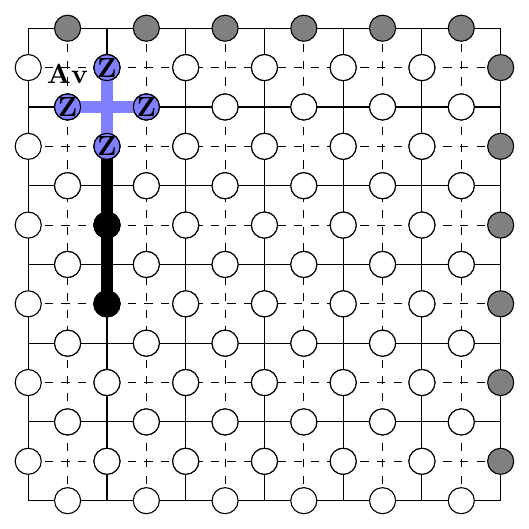
\begin{tikzpicture}
			% Draw dashed lines
			\foreach \i in {-3,-2.5,...,3}
			{
				\draw[dashed] (\i,-3) -- (\i,3);
			}
			\foreach \j in {-3,-2.5,...,3}
			{
				\draw[dashed] (-3,\j) -- (3,\j);
			}
			
			
			
			% Draw solid grid and nodes with circles in the middle of each side
			\draw[step=1cm] (-3,-3) grid (3,3);
			\foreach \i in {-2.5,...,2.5}
			{
				\foreach \j in {-2.5,...,2.5}
				{
					
					
					\begin{scope}[transform canvas={xshift=\i cm,yshift=\j cm}]
						\node[right,xshift=0.2cm,yshift=0.4cm] {};
						% Convert \j and \i to integers
						\pgfmathtruncatemacro{\intj}{\j}
						\pgfmathtruncatemacro{\inti}{\i}
						
						% Draw circles at the midpoints of each side
						\ifnum\intj=2
						\draw node[draw,circle,fill=gray] at (0,0.5) {};
						\else
						\draw node[draw,circle,fill=white] at (0,0.5) {};
						\fi
						
						\ifnum\inti=2
						\draw node[draw,circle,fill=gray] at (0.5,0) {};
						\else
						\draw node[draw,circle,fill=white] at (0.5,0) {};
						\fi
						
						\draw node[draw,circle,fill=white] at (0,-0.5) {};
						\draw node[draw,circle,fill=white] at (-0.5,0) {};
					\end{scope}
				}
			}
			
			\foreach \i in {-2,...,-2}
			{
				\draw[black, line width=1.5mm] (\i,-0.5) -- (\i,1.5);
				\node[draw, circle, fill=black] at (\i,-0.5) {};
				\node[draw, circle, fill=black] at (\i,0.5) {};
				
				\draw[blue!50, line width=1.5mm] (\i,1.5) -- (\i,2.5);
				\node[draw, circle, fill=blue!50,label=center:\textbf{Z}] at (\i,1.5) {};
				\node[draw, circle, fill=blue!50,label=center:\textbf{Z}] at (\i,2.5) {};
				
				
			}
			
			\foreach \j in {2,...,2}
			{
				
				\draw[blue!50, line width=1.5mm] (-2.5, \j) -- (-1.5, \j);
				
				\draw node[draw,circle,fill=blue!50,label=center:\textbf{Z},label=north:\textbf{Av}] at (-2.5,\j) {};
				\draw node[draw,circle,fill=blue!50,label=center:\textbf{Z}] at (-1.5,\j) {};
				
			}
			
			
		\end{tikzpicture}
	\end{center}
	
	\caption{Operator $Av$ applied on an open string of occupied edges.}
	\label{fig:Aveigen2}
\end{figure}




\begin{figure}
	
\begin{center}
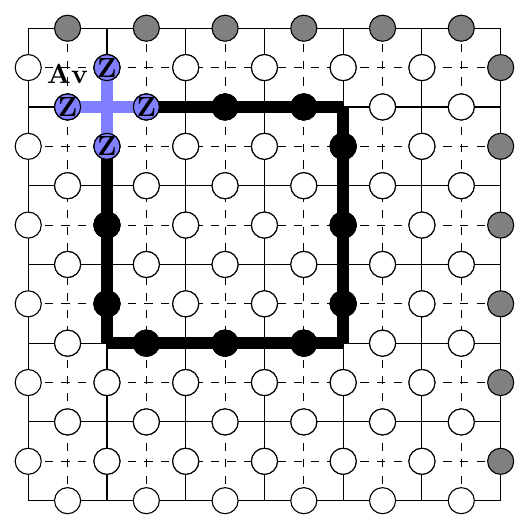
\begin{tikzpicture}
	% Draw dashed lines
	\foreach \i in {-3,-2.5,...,3}
	{
		\draw[dashed] (\i,-3) -- (\i,3);
	}
	\foreach \j in {-3,-2.5,...,3}
	{
		\draw[dashed] (-3,\j) -- (3,\j);
	}
	
	
	
	% Draw solid grid and nodes with circles in the middle of each side
	\draw[step=1cm] (-3,-3) grid (3,3);
	\foreach \i in {-2.5,...,2.5}
	{
		\foreach \j in {-2.5,...,2.5}
		{
			
			
			\begin{scope}[transform canvas={xshift=\i cm,yshift=\j cm}]
				\node[right,xshift=0.2cm,yshift=0.4cm] {};
				% Convert \j and \i to integers
				\pgfmathtruncatemacro{\intj}{\j}
				\pgfmathtruncatemacro{\inti}{\i}
				
				% Draw circles at the midpoints of each side
				\ifnum\intj=2
				\draw node[draw,circle,fill=gray] at (0,0.5) {};
				\else
				\draw node[draw,circle,fill=white] at (0,0.5) {};
				\fi
				
				\ifnum\inti=2
				\draw node[draw,circle,fill=gray] at (0.5,0) {};
				\else
				\draw node[draw,circle,fill=white] at (0.5,0) {};
				\fi
				
				\draw node[draw,circle,fill=white] at (0,-0.5) {};
				\draw node[draw,circle,fill=white] at (-0.5,0) {};
			\end{scope}
		}
	}
	
	\foreach \i in {-2,...,-2}
	{
		\draw[black, line width=1.5mm] (\i,-1) -- (\i,1.5);
		\node[draw, circle, fill=black] at (\i,-0.5) {};
		\node[draw, circle, fill=black] at (\i,0.5) {};
		
		\draw[blue!50, line width=1.5mm] (\i,1.5) -- (\i,2.5);
		\node[draw, circle, fill=blue!50,label=center:\textbf{Z}] at (\i,1.5) {};
		\node[draw, circle, fill=blue!50,label=center:\textbf{Z}] at (\i,2.5) {};
		
		
	}
	
	\foreach \j in {2,...,2}
	{
		
		\draw[blue!50, line width=1.5mm] (-2.5, \j) -- (-1.5, \j);
		
		
		\draw[black, line width=1.5mm] (-1.5, \j) -- (1, \j);
		\draw node[draw,circle,fill=black] at (-0.5,\j) {};
		\draw node[draw,circle,fill=black] at (0.5,\j) {};
		\draw node[draw,circle,fill=blue!50,label=center:\textbf{Z},label=north:\textbf{Av}] at (-2.5,\j) {};
		\draw node[draw,circle,fill=blue!50,label=center:\textbf{Z}] at (-1.5,\j) {};
		
	}
	
	
	\foreach \i in {1,...,1}
	{
		\draw[black, line width=1.5mm] (\i,-1) -- (\i,2);
		\node[draw, circle, fill=black] at (\i,-0.5) {};
		\node[draw, circle, fill=black] at (\i,0.5) {};
		\draw node[draw,circle,fill=black] at (\i,1.5) {};
		
	}
	
	\foreach \j in {-1,...,-1}
	{
		\draw[black, line width=1.5mm] (-2, \j) -- (1, \j);
		\draw node[draw,circle,fill=black] at (0.5,\j) {};
		\draw node[draw,circle,fill=black] at (-0.5,\j) {};
		\draw node[draw,circle,fill=black] at (-1.5,\j) {};
	}
	
	
\end{tikzpicture}
\end{center}

\caption{String of occupied edges closed on an operator $Av$.}
\label{fig:Aveigen}
\end{figure}
		
In a more formal notation what we are stating is that:

\begin{center}
	$\prod_{i=1}^{4} \sigma_{i}^{z} |\psi\rangle = +1 |\psi\rangle$. 
\end{center}

If we consider only closed loops, we can identify different configurations having such characteristic. The illustrations in figure 1.6 show some examples of them.
Each of these loops, having such characteristics, is an eigenstate for $Av$ since, no matter how I locally apply $Av$, I will always preserve the sign of the state. 

%drawings 4 types of loops


\begin{figure}
	
	\begin{center}
		
		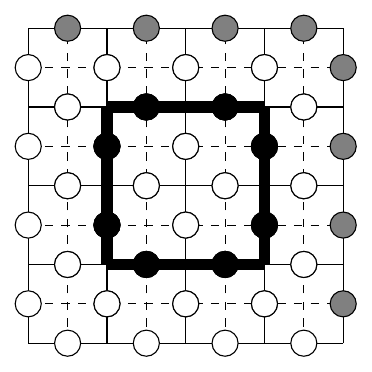
\begin{tikzpicture}
			% Draw dashed lines
			\foreach \i in {-2,-1.5,...,2}
			{
				\draw[dashed] (\i,-2) -- (\i,2);
			}
			\foreach \j in {-2,-1.5,...,2}
			{
				\draw[dashed] (-2,\j) -- (2,\j);
			}
			
			% Draw solid grid and nodes with circles in the middle of each side
			\draw[step=1cm] (-2,-2) grid (2,2);
			\foreach \i in {-1.5,...,1.5}
			{
				\foreach \j in {-1.5,...,1.5}
				{
					\begin{scope}[transform canvas={xshift=\i cm,yshift=\j cm}]
						\node[right,xshift=0.2cm,yshift=0.4cm] {};
						% Convert \j and \i to integers
						\pgfmathtruncatemacro{\intj}{\j}
						\pgfmathtruncatemacro{\inti}{\i}
						
						% Draw circles at the midpoints of each side
						\ifnum\intj=1
						\draw node[draw,circle,fill=gray] at (0,0.5) {};
						\else
						\draw node[draw,circle,fill=white] at (0,0.5) {};
						\fi
						
						\ifnum\inti=1
						\draw node[draw,circle,fill=gray] at (0.5,0) {};
						\else
						\draw node[draw,circle,fill=white] at (0.5,0) {};
						\fi
						
						\draw node[draw,circle,fill=white] at (0,-0.5) {};
						\draw node[draw,circle,fill=white] at (-0.5,0) {};
					\end{scope}
				}
			}
			
			\foreach \i in {-1,...,-1}
			{
				\draw[black, line width=1.5mm] (\i,-1) -- (\i,1);
				\node[draw, circle, fill=black] at (\i,-0.5) {};
				\node[draw, circle, fill=black] at (\i,0.5) {};	
				
			}
			
			\foreach \i in {1,...,1}
			{
				\draw[black, line width=1.5mm] (\i,-1) -- (\i,1);
				\node[draw, circle, fill=black] at (\i,-0.5) {};
				\node[draw, circle, fill=black] at (\i,0.5) {};	
				
			}
			
			\foreach \j in {1,...,1}
			{
				\draw[black, line width=1.5mm] (-1,\j) -- (1,\j);
				\node[draw, circle, fill=black] at (-0.5,\j) {};
				\node[draw, circle, fill=black] at (0.5,\j) {};		
				
			}
			
			\foreach \j in {-1,...,-1}
			{
				\draw[black, line width=1.5mm] (-1,\j) -- (1,\j);
				\node[draw, circle, fill=black] at (-0.5,\j) {};
				\node[draw, circle, fill=black] at (0.5,\j) {};		
				
			}
			
			
		\end{tikzpicture}
		
	\end{center}
	
	\vspace{1cm} 
	
	\begin{center}
		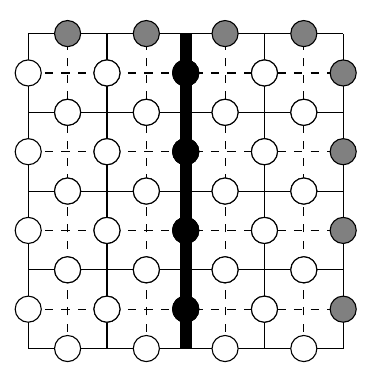
\begin{tikzpicture}
			% Draw dashed lines
			\foreach \i in {-2,-1.5,...,2}
			{
				\draw[dashed] (\i,-2) -- (\i,2);
			}
			\foreach \j in {-2,-1.5,...,2}
			{
				\draw[dashed] (-2,\j) -- (2,\j);
			}
			
			% Draw solid grid and nodes with circles in the middle of each side
			\draw[step=1cm] (-2,-2) grid (2,2);
			\foreach \i in {-1.5,...,1.5}
			{
				\foreach \j in {-1.5,...,1.5}
				{
					\begin{scope}[transform canvas={xshift=\i cm,yshift=\j cm}]
						\node[right,xshift=0.2cm,yshift=0.4cm] {};
						% Convert \j and \i to integers
						\pgfmathtruncatemacro{\intj}{\j}
						\pgfmathtruncatemacro{\inti}{\i}
						
						% Draw circles at the midpoints of each side
						\ifnum\intj=1
						\draw node[draw,circle,fill=gray] at (0,0.5) {};
						\else
						\draw node[draw,circle,fill=white] at (0,0.5) {};
						\fi
						
						\ifnum\inti=1
						\draw node[draw,circle,fill=gray] at (0.5,0) {};
						\else
						\draw node[draw,circle,fill=white] at (0.5,0) {};
						\fi
						
						\draw node[draw,circle,fill=white] at (0,-0.5) {};
						\draw node[draw,circle,fill=white] at (-0.5,0) {};
					\end{scope}
				}
			}
			
			\foreach \i in {0,...,0}
			{
				\draw[black, line width=1.5mm] (\i,-2) -- (\i,2);
				\node[draw, circle, fill=black] at (\i,-0.5) {};
				\node[draw, circle, fill=black] at (\i,0.5) {};		
				\node[draw, circle, fill=black] at (\i,-1.5) {};
				\node[draw, circle, fill=black] at (\i,1.5) {};		
				
			}
			
			
		\end{tikzpicture}		
	\end{center}
	
	\vspace{1cm} 
	
	\begin{center}
		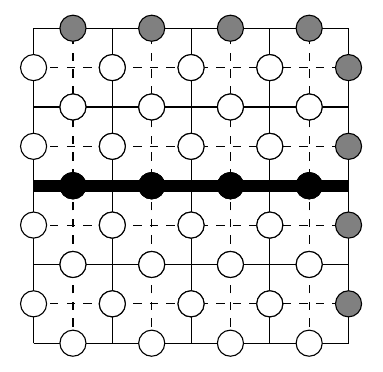
\begin{tikzpicture}
			% Draw dashed lines
			\foreach \i in {-2,-1.5,...,2}
			{
				\draw[dashed] (\i,-2) -- (\i,2);
			}
			\foreach \j in {-2,-1.5,...,2}
			{
				\draw[dashed] (-2,\j) -- (2,\j);
			}
			
			% Draw solid grid and nodes with circles in the middle of each side
			\draw[step=1cm] (-2,-2) grid (2,2);
			\foreach \i in {-1.5,...,1.5}
			{
				\foreach \j in {-1.5,...,1.5}
				{
					\begin{scope}[transform canvas={xshift=\i cm,yshift=\j cm}]
						\node[right,xshift=0.2cm,yshift=0.4cm] {};
						% Convert \j and \i to integers
						\pgfmathtruncatemacro{\intj}{\j}
						\pgfmathtruncatemacro{\inti}{\i}
						
						% Draw circles at the midpoints of each side
						\ifnum\intj=1
						\draw node[draw,circle,fill=gray] at (0,0.5) {};
						\else
						\draw node[draw,circle,fill=white] at (0,0.5) {};
						\fi
						
						\ifnum\inti=1
						\draw node[draw,circle,fill=gray] at (0.5,0) {};
						\else
						\draw node[draw,circle,fill=white] at (0.5,0) {};
						\fi
						
						\draw node[draw,circle,fill=white] at (0,-0.5) {};
						\draw node[draw,circle,fill=white] at (-0.5,0) {};
					\end{scope}
				}
			}
			
			\foreach \j in {0,...,0}
			{
				\draw[black, line width=1.5mm] (-2,\j) -- (2,\j);
				\node[draw, circle, fill=black] at (-0.5,\j) {};
				\node[draw, circle, fill=black] at (0.5,\j) {};		
				\node[draw, circle, fill=black] at (-1.5,\j) {};
				\node[draw, circle, fill=black] at (1.5,\j) {};		
				
			}
			
			
		\end{tikzpicture}
	\end{center}
	
	\vspace{1cm} 
	
	\begin{center}
		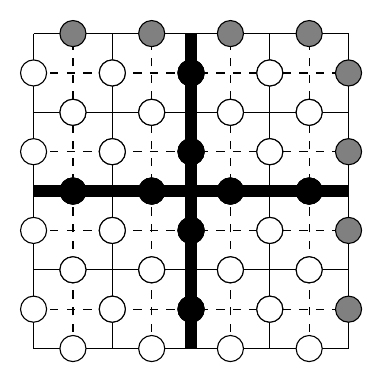
\begin{tikzpicture}
			% Draw dashed lines
			\foreach \i in {-2,-1.5,...,2}
			{
				\draw[dashed] (\i,-2) -- (\i,2);
			}
			\foreach \j in {-2,-1.5,...,2}
			{
				\draw[dashed] (-2,\j) -- (2,\j);
			}
			
			% Draw solid grid and nodes with circles in the middle of each side
			\draw[step=1cm] (-2,-2) grid (2,2);
			\foreach \i in {-1.5,...,1.5}
			{
				\foreach \j in {-1.5,...,1.5}
				{
					\begin{scope}[transform canvas={xshift=\i cm,yshift=\j cm}]
						\node[right,xshift=0.2cm,yshift=0.4cm] {};
						% Convert \j and \i to integers
						\pgfmathtruncatemacro{\intj}{\j}
						\pgfmathtruncatemacro{\inti}{\i}
						
						% Draw circles at the midpoints of each side
						\ifnum\intj=1
						\draw node[draw,circle,fill=gray] at (0,0.5) {};
						\else
						\draw node[draw,circle,fill=white] at (0,0.5) {};
						\fi
						
						\ifnum\inti=1
						\draw node[draw,circle,fill=gray] at (0.5,0) {};
						\else
						\draw node[draw,circle,fill=white] at (0.5,0) {};
						\fi
						
						\draw node[draw,circle,fill=white] at (0,-0.5) {};
						\draw node[draw,circle,fill=white] at (-0.5,0) {};
					\end{scope}
				}
			}
			
			
			\foreach \i in {0,...,0}
			{
				\draw[black, line width=1.5mm] (\i,-2) -- (\i,2);
				\node[draw, circle, fill=black] at (\i,-0.5) {};
				\node[draw, circle, fill=black] at (\i,0.5) {};		
				\node[draw, circle, fill=black] at (\i,-1.5) {};
				\node[draw, circle, fill=black] at (\i,1.5) {};		
				
			}
			
			\foreach \j in {0,...,0}
			{
				\draw[black, line width=1.5mm] (-2,\j) -- (2,\j);
				\node[draw, circle, fill=black] at (-0.5,\j) {};
				\node[draw, circle, fill=black] at (0.5,\j) {};		
				\node[draw, circle, fill=black] at (-1.5,\j) {};
				\node[draw, circle, fill=black] at (1.5,\j) {};		
				
			}
			
			
		\end{tikzpicture}		
	\end{center}
	
	\caption{Examples of closed loops yielding $+1$ eigenvalue for $Av$}
	\label{fig:Loops}
\end{figure}


Now we focus on constraint (2). We want to apply the plaquette operator $Bp$ only to eigenstates of $Av$, which we have determined above. The illustration in figure 1.7 shows an example of how to do it in practice with one of the eigenstates of $Av$.
Notice that, after the transformation, we do always end up in a valid eigenstate of $Av$ but the new state $|\psi'\rangle$ is not an eigenstate of $Bp$ by itself.

%drawings Bp applied to loops
\begin{figure}
	
	\begin{center}
		
		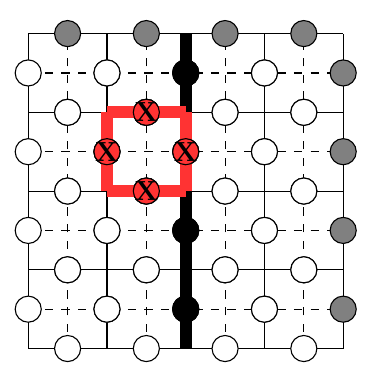
\begin{tikzpicture}
			% Draw dashed lines
			\foreach \i in {-2,-1.5,...,2}
			{
				\draw[dashed] (\i,-2) -- (\i,2);
			}
			\foreach \j in {-2,-1.5,...,2}
			{
				\draw[dashed] (-2,\j) -- (2,\j);
			}
			
			% Draw solid grid and nodes with circles in the middle of each side
			\draw[step=1cm] (-2,-2) grid (2,2);
			\foreach \i in {-1.5,...,1.5}
			{
				\foreach \j in {-1.5,...,1.5}
				{
					\begin{scope}[transform canvas={xshift=\i cm,yshift=\j cm}]
						\node[right,xshift=0.2cm,yshift=0.4cm] {};
						% Convert \j and \i to integers
						\pgfmathtruncatemacro{\intj}{\j}
						\pgfmathtruncatemacro{\inti}{\i}
						
						% Draw circles at the midpoints of each side
						\ifnum\intj=1
						\draw node[draw,circle,fill=gray] at (0,0.5) {};
						\else
						\draw node[draw,circle,fill=white] at (0,0.5) {};
						\fi
						
						\ifnum\inti=1
						\draw node[draw,circle,fill=gray] at (0.5,0) {};
						\else
						\draw node[draw,circle,fill=white] at (0.5,0) {};
						\fi
						
						\draw node[draw,circle,fill=white] at (0,-0.5) {};
						\draw node[draw,circle,fill=white] at (-0.5,0) {};
					\end{scope}
				}
			}
			
			\foreach \i in {0,...,0}
			{
				\draw[black, line width=1.5mm] (\i,-2) -- (\i,0);
				\draw[red!80, line width=1.5mm] (\i,0) -- (\i,1);
				\draw[black, line width=1.5mm] (\i,1) -- (\i,2);
				\node[draw, circle, fill=black] at (\i,-0.5) {};
				\node[draw, circle, fill=red!80,label = center:\textbf{X}] at (\i,0.5) {};
				\node[draw, circle, fill=black] at (\i,-1.5) {};
				\node[draw, circle, fill=black] at (\i,1.5) {};		
				
			}
			
			\foreach \i in {-1,...,-1}
			{
				
				\draw[red!80, line width=1.5mm] (\i,0) -- (\i,1);
				\node[draw, circle, fill=red!80,label = center:\textbf{X}] at (\i,0.5) {};
				
			}
			
			\foreach \j in {0,...,0}
			{
				\draw[red!80, line width=1.5mm] (-1,\j) -- (0,\j);
				\node[draw, circle, fill=red!80,label = center:\textbf{X}] at (-0.5,\j) {};		
				
			}
			
			\foreach \j in {1,...,1}
			{
				\draw[red!80, line width=1.5mm] (-1,\j) -- (0,\j);
				\node[draw, circle, fill=red!80,label = center:\textbf{X}] at (-0.5,\j) {};	
				
			}
			
			
		\end{tikzpicture}
		
		
		
		\vspace{1cm} 
		
		
		
		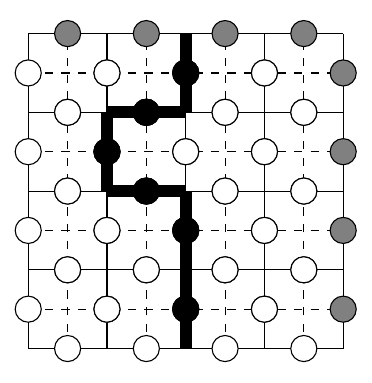
\begin{tikzpicture}
			% Draw dashed lines
			\foreach \i in {-2,-1.5,...,2}
			{
				\draw[dashed] (\i,-2) -- (\i,2);
			}
			\foreach \j in {-2,-1.5,...,2}
			{
				\draw[dashed] (-2,\j) -- (2,\j);
			}
			
			% Draw solid grid and nodes with circles in the middle of each side
			\draw[step=1cm] (-2,-2) grid (2,2);
			\foreach \i in {-1.5,...,1.5}
			{
				\foreach \j in {-1.5,...,1.5}
				{
					\begin{scope}[transform canvas={xshift=\i cm,yshift=\j cm}]
						\node[right,xshift=0.2cm,yshift=0.4cm] {};
						% Convert \j and \i to integers
						\pgfmathtruncatemacro{\intj}{\j}
						\pgfmathtruncatemacro{\inti}{\i}
						
						% Draw circles at the midpoints of each side
						\ifnum\intj=1
						\draw node[draw,circle,fill=gray] at (0,0.5) {};
						\else
						\draw node[draw,circle,fill=white] at (0,0.5) {};
						\fi
						
						\ifnum\inti=1
						\draw node[draw,circle,fill=gray] at (0.5,0) {};
						\else
						\draw node[draw,circle,fill=white] at (0.5,0) {};
						\fi
						
						\draw node[draw,circle,fill=white] at (0,-0.5) {};
						\draw node[draw,circle,fill=white] at (-0.5,0) {};
					\end{scope}
				}
			}
			
			\foreach \i in {0,...,0}
			{
				\draw[black, line width=1.5mm] (\i,-2) -- (\i,0);
				\draw[black, line width=1.5mm] (\i,1) -- (\i,2);
				\node[draw, circle, fill=black] at (\i,-0.5) {};
				
				\node[draw, circle, fill=black] at (\i,-1.5) {};
				\node[draw, circle, fill=black] at (\i,1.5) {};		
				
			}
			
			\foreach \i in {-1,...,-1}
			{
				
				\draw[black, line width=1.5mm] (\i,0) -- (\i,1);
				\node[draw, circle, fill=black] at (\i,0.5) {};
				
			}
			
			\foreach \j in {0,...,0}
			{
				\draw[black, line width=1.5mm] (-1,\j) -- (0,\j);
				\node[draw, circle, fill=black] at (-0.5,\j) {};		
				
			}
			
			\foreach \j in {1,...,1}
			{
				\draw[black, line width=1.5mm] (-1,\j) -- (0,\j);
				\node[draw, circle, fill=black] at (-0.5,\j) {};
				\node[draw, circle, black] at (-0.5,\j) {};	
				
			}
			
			
		\end{tikzpicture}	

	\end{center}

\caption{Examples of $Bp$ to a closed loop.}
\label{fig:applyBp}
\end{figure}


Furthermore, any new configuration that we obtain through the application of the plaquette operator to an eigenstate of $Av$ simply yields one of the possible permutations of the edges of the initial state, provided that the topological characteristics of the loop are preserved.

This means that if we firstly partition the eigenstates of $Av$ in the following fours classes: 

\begin{enumerate}
	\item class 0 : contains all closed loops and thus the null state,
	this is because all of the closed loops can be continuously deformed into a null state;
	
	\item class 1 : contains loops that wind all the way around the horizontal dimension of the torus and their permutations;
	
	\item class 2 : contains loops that wind all the way around the vertical dimension of the torus and their permutations;
	
	\item class 3 : contains loops that wind all the way around both dimension of the torus and their permutations. Notice that the vertical loop must be taken on the dual lattice to yield a valid configuration.
	
\end{enumerate}

Then, applying a plaquette operator to any of the eigenstates belonging to one of the classes above must yield an eigenstate that lies in the same class. This is formally expressed by stating that the class is invariant under the action of the operator $Bp$. 

\begin{proposition} (Invariance under $Bp$) The four classes of eigenstates of $Av$ are invariant under the action of the $Bp$ operator. 
\end{proposition}

We can prove that the above definition holds by means of counterexamples. \newline



%drawing loop chiuso ma unito da Bp
\begin{figure}
	
	\begin{center}	
		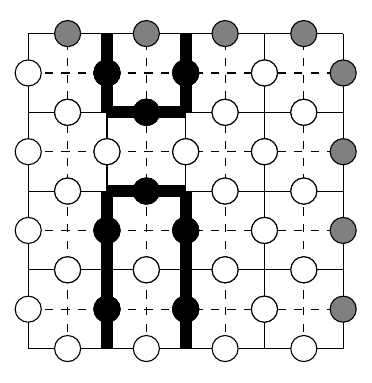
\begin{tikzpicture}
			% Draw dashed lines
			\foreach \i in {-2,-1.5,...,2}
			{
				\draw[dashed] (\i,-2) -- (\i,2);
			}
			\foreach \j in {-2,-1.5,...,2}
			{
				\draw[dashed] (-2,\j) -- (2,\j);
			}
			
			% Draw solid grid and nodes with circles in the middle of each side
			\draw[step=1cm] (-2,-2) grid (2,2);
			\foreach \i in {-1.5,...,1.5}
			{
				\foreach \j in {-1.5,...,1.5}
				{
					\begin{scope}[transform canvas={xshift=\i cm,yshift=\j cm}]
						\node[right,xshift=0.2cm,yshift=0.4cm] {};
						% Convert \j and \i to integers
						\pgfmathtruncatemacro{\intj}{\j}
						\pgfmathtruncatemacro{\inti}{\i}
						
						% Draw circles at the midpoints of each side
						\ifnum\intj=1
						\draw node[draw,circle,fill=gray] at (0,0.5) {};
						\else
						\draw node[draw,circle,fill=white] at (0,0.5) {};
						\fi
						
						\ifnum\inti=1
						\draw node[draw,circle,fill=gray] at (0.5,0) {};
						\else
						\draw node[draw,circle,fill=white] at (0.5,0) {};
						\fi
						
						\draw node[draw,circle,fill=white] at (0,-0.5) {};
						\draw node[draw,circle,fill=white] at (-0.5,0) {};
					\end{scope}
				}
			}
			
			\foreach \i in {0,...,0}
			{
				\draw[black, line width=1.5mm] (\i,-2) -- (\i,0);
				\draw[black, line width=1.5mm] (\i,1) -- (\i,2);
				\node[draw, circle, fill=black] at (\i,-0.5) {};
				
				\node[draw, circle, fill=black] at (\i,-1.5) {};
				\node[draw, circle, fill=black] at (\i,1.5) {};		
				
			}
			
			\foreach \i in {-1,...,-1}
			{
				\draw[black, line width=1.5mm] (\i,-2) -- (\i,0);
				\draw[black, line width=1.5mm] (\i,1) -- (\i,2);
				\node[draw, circle, fill=black] at (\i,-0.5) {};
				
				\node[draw, circle, fill=black] at (\i,-1.5) {};
				\node[draw, circle, fill=black] at (\i,1.5) {};		
				
			}
			
			\foreach \i in {-1,...,-1}
			{
				
				\draw[black, line width=1.5mm] (\i,1) -- (\i,2);
				\node[draw, circle, fill=black] at (\i,1.5) {};
				
			}
			
			\foreach \j in {0,...,0}
			{
				\draw[black, line width=1.5mm] (-1,\j) -- (0,\j);
				\node[draw, circle, fill=black] at (-0.5,\j) {};		
				
			}
			
			\foreach \j in {1,...,1}
			{
				\draw[black, line width=1.5mm] (-1,\j) -- (0,\j);
				\node[draw, circle, fill=black] at (-0.5,\j) {};
				\node[draw, circle, black] at (-0.5,\j) {};	
				
			}
			
			
		\end{tikzpicture}	
		
		\vspace{1cm} 
		
		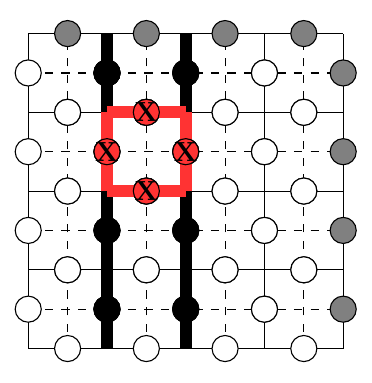
\begin{tikzpicture}
			% Draw dashed lines
			\foreach \i in {-2,-1.5,...,2}
			{
				\draw[dashed] (\i,-2) -- (\i,2);
			}
			\foreach \j in {-2,-1.5,...,2}
			{
				\draw[dashed] (-2,\j) -- (2,\j);
			}
			
			% Draw solid grid and nodes with circles in the middle of each side
			\draw[step=1cm] (-2,-2) grid (2,2);
			\foreach \i in {-1.5,...,1.5}
			{
				\foreach \j in {-1.5,...,1.5}
				{
					\begin{scope}[transform canvas={xshift=\i cm,yshift=\j cm}]
						\node[right,xshift=0.2cm,yshift=0.4cm] {};
						% Convert \j and \i to integers
						\pgfmathtruncatemacro{\intj}{\j}
						\pgfmathtruncatemacro{\inti}{\i}
						
						% Draw circles at the midpoints of each side
						\ifnum\intj=1
						\draw node[draw,circle,fill=gray] at (0,0.5) {};
						\else
						\draw node[draw,circle,fill=white] at (0,0.5) {};
						\fi
						
						\ifnum\inti=1
						\draw node[draw,circle,fill=gray] at (0.5,0) {};
						\else
						\draw node[draw,circle,fill=white] at (0.5,0) {};
						\fi
						
						\draw node[draw,circle,fill=white] at (0,-0.5) {};
						\draw node[draw,circle,fill=white] at (-0.5,0) {};
					\end{scope}
				}
			}
			
			\foreach \i in {0,...,0}
			{
				\draw[black, line width=1.5mm] (\i,-2) -- (\i,0);
				\draw[black, line width=1.5mm] (\i,1) -- (\i,2);
				\node[draw, circle, fill=black] at (\i,-0.5) {};
				
				\node[draw, circle, fill=black] at (\i,-1.5) {};
				\node[draw, circle, fill=black] at (\i,1.5) {};		
				
				\draw[red!80, line width=1.5mm] (\i,0) -- (\i,1);
				\node[draw, circle, fill=red!80, label = center:\textbf{X}] at (\i,0.5) {};		
				
			}
			
			\foreach \i in {-1,...,-1}
			{
				\draw[black, line width=1.5mm] (\i,-2) -- (\i,0);
				\draw[black, line width=1.5mm] (\i,1) -- (\i,2);
				\node[draw, circle, fill=black] at (\i,-0.5) {};
				
				\node[draw, circle, fill=black] at (\i,-1.5) {};
				\node[draw, circle, fill=black] at (\i,1.5) {};		
				
				
				
			}
			
			\foreach \i in {-1,...,-1}
			{
				
				\draw[black, line width=1.5mm] (\i,1) -- (\i,2);
				\draw[red!80, line width=1.5mm] (\i,0) -- (\i,1);
				\node[draw, circle, fill=black] at (\i,1.5) {};
				\node[draw, circle, fill=red!80,label = center:\textbf{X}] at (\i,0.5) {};
				
			}
			
			\foreach \j in {0,...,0}
			{
				\draw[red!80, line width=1.5mm] (-1,\j) -- (0,\j);
				\node[draw, circle, fill=red!80,label = center:\textbf{X}] at (-0.5,\j) {};		
				
			}
			
			\foreach \j in {1,...,1}
			{
				\draw[red!80, line width=1.5mm] (-1,\j) -- (0,\j);
				\node[draw, circle, fill=red!80,label = center:\textbf{X}] at (-0.5,\j) {};
				
				
			}
			
			
		\end{tikzpicture}	
		
		\vspace{1cm} 
		
		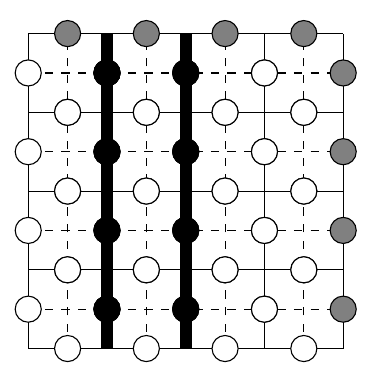
\begin{tikzpicture}
			% Draw dashed lines
			\foreach \i in {-2,-1.5,...,2}
			{
				\draw[dashed] (\i,-2) -- (\i,2);
			}
			\foreach \j in {-2,-1.5,...,2}
			{
				\draw[dashed] (-2,\j) -- (2,\j);
			}
			
			% Draw solid grid and nodes with circles in the middle of each side
			\draw[step=1cm] (-2,-2) grid (2,2);
			\foreach \i in {-1.5,...,1.5}
			{
				\foreach \j in {-1.5,...,1.5}
				{
					\begin{scope}[transform canvas={xshift=\i cm,yshift=\j cm}]
						\node[right,xshift=0.2cm,yshift=0.4cm] {};
						% Convert \j and \i to integers
						\pgfmathtruncatemacro{\intj}{\j}
						\pgfmathtruncatemacro{\inti}{\i}
						
						% Draw circles at the midpoints of each side
						\ifnum\intj=1
						\draw node[draw,circle,fill=gray] at (0,0.5) {};
						\else
						\draw node[draw,circle,fill=white] at (0,0.5) {};
						\fi
						
						\ifnum\inti=1
						\draw node[draw,circle,fill=gray] at (0.5,0) {};
						\else
						\draw node[draw,circle,fill=white] at (0.5,0) {};
						\fi
						
						\draw node[draw,circle,fill=white] at (0,-0.5) {};
						\draw node[draw,circle,fill=white] at (-0.5,0) {};
					\end{scope}
				}
			}
			
			\foreach \i in {0,...,0}
			{
				\draw[black, line width=1.5mm] (\i,-2) -- (\i,0);
				\draw[black, line width=1.5mm] (\i,1) -- (\i,2);
				\node[draw, circle, fill=black] at (\i,-0.5) {};
				
				\node[draw, circle, fill=black] at (\i,-1.5) {};
				\node[draw, circle, fill=black] at (\i,1.5) {};		
				
				\draw[black, line width=1.5mm] (\i,0) -- (\i,1);
				\node[draw, circle, fill=black] at (\i,0.5) {};		
				
			}
			
			\foreach \i in {-1,...,-1}
			{
				\draw[black, line width=1.5mm] (\i,-2) -- (\i,0);
				\draw[black, line width=1.5mm] (\i,1) -- (\i,2);
				\node[draw, circle, fill=black] at (\i,-0.5) {};
				
				\node[draw, circle, fill=black] at (\i,-1.5) {};
				\node[draw, circle, fill=black] at (\i,1.5) {};		
				
				
				
			}
			
			\foreach \i in {-1,...,-1}
			{
				
				\draw[black, line width=1.5mm] (\i,1) -- (\i,2);
				\draw[black, line width=1.5mm] (\i,0) -- (\i,1);
				\node[draw, circle, fill=black] at (\i,1.5) {};
				\node[draw, circle, fill=black] at (\i,0.5) {};
				
			}
			
			
			
		\end{tikzpicture}	
		

	\end{center}

\caption{Apply $Bp$ to a closed loop.}
\label{fig:Bpstrano}
\end{figure}

If we take the loop illustrated in figure 1.8 and close it by means of a plaquette operator as illustrated, we would be brought to believe that there indeed exist a way to apply the operator $Bp$ such that we exit class zero and land in class 1. Though, this is not possible. \newline
In fact, we can show the impossibility of the above action by defining two topological indeces to label the four categories of eigenstates. These indeces can assume values in $\mathbb{Z}_2=\{\overline{0},\overline{1} \}$, whose elements respectively represent the 'sets' of even and odd numbers. In our context such numerosities identify the number of vertical and horizontal loops of a configuration intersecting the vertical and horizontal dimensions of the torus (figure 1.9).

The above indeces can be expressed more clearly as follows: 

\begin{center}
	$n_x= (number \ of \ vertical \ intersections)mod2 = 
	\begin{cases} 
		0mod2 \\
		1mod2  
	\end{cases}$ 
\end{center}
\begin{center}
	$n_y= (number \ of \ horizontal \ intersections)mod2 =\begin{cases} 
		0mod2 \\
		1mod2  
	\end{cases}$ 
\end{center}


in order to create a correspondence with the actual definition of the torus over $(\mathbb{Z}$ x $\mathbb{Z})$. 
%We only change the representatives of the elements $\{\overline{0},\overline{1} \}$ in the intermediate step. \newline

In total our classes are going to be wider than expected; we can label them as : $(\overline{0},\overline{0} )$, $(\overline{0},\overline{1} )$, $(\overline{1},\overline{0})$, $(\overline{1},\overline{1})$.\newline

For example, if we take again the configuration in figure 1.9, we have 1 vertical intersection and 1 horizontal intersection, therefore we are in the class three indexed by $n_x=1mod2$ and $n_y=1mod2$, which is labelled as $(\overline{1},\overline{1})$. This would have been true for any odd number of vertical and horizintal intersections, since they all fall in the set of numbers given by $1mod2$.


%drawing 1 vertical 1 hor
\begin{figure}
	\begin{center}
	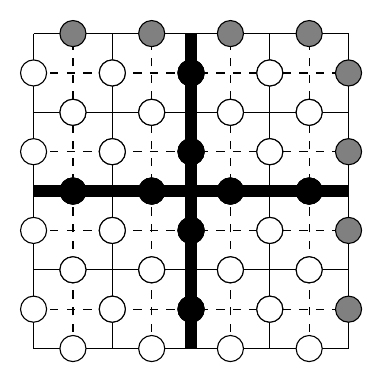
\begin{tikzpicture}
		% Draw dashed lines
		\foreach \i in {-2,-1.5,...,2}
		{
			\draw[dashed] (\i,-2) -- (\i,2);
		}
		\foreach \j in {-2,-1.5,...,2}
		{
			\draw[dashed] (-2,\j) -- (2,\j);
		}
		
		% Draw solid grid and nodes with circles in the middle of each side
		\draw[step=1cm] (-2,-2) grid (2,2);
		\foreach \i in {-1.5,...,1.5}
		{
			\foreach \j in {-1.5,...,1.5}
			{
				\begin{scope}[transform canvas={xshift=\i cm,yshift=\j cm}]
					\node[right,xshift=0.2cm,yshift=0.4cm] {};
					% Convert \j and \i to integers
					\pgfmathtruncatemacro{\intj}{\j}
					\pgfmathtruncatemacro{\inti}{\i}
					
					% Draw circles at the midpoints of each side
					\ifnum\intj=1
					\draw node[draw,circle,fill=gray] at (0,0.5) {};
					\else
					\draw node[draw,circle,fill=white] at (0,0.5) {};
					\fi
					
					\ifnum\inti=1
					\draw node[draw,circle,fill=gray] at (0.5,0) {};
					\else
					\draw node[draw,circle,fill=white] at (0.5,0) {};
					\fi
					
					\draw node[draw,circle,fill=white] at (0,-0.5) {};
					\draw node[draw,circle,fill=white] at (-0.5,0) {};
				\end{scope}
			}
		}
		
		
		\foreach \i in {0,...,0}
		{
			\draw[black, line width=1.5mm] (\i,-2) -- (\i,2);
			\node[draw, circle, fill=black] at (\i,-0.5) {};
			\node[draw, circle, fill=black] at (\i,0.5) {};		
			\node[draw, circle, fill=black] at (\i,-1.5) {};
			\node[draw, circle, fill=black] at (\i,1.5) {};		
			
		}
		
		\foreach \j in {0,...,0}
		{
			\draw[black, line width=1.5mm] (-2,\j) -- (2,\j);
			\node[draw, circle, fill=black] at (-0.5,\j) {};
			\node[draw, circle, fill=black] at (0.5,\j) {};		
			\node[draw, circle, fill=black] at (-1.5,\j) {};
			\node[draw, circle, fill=black] at (1.5,\j) {};		
			
		}
		
		
	\end{tikzpicture}		
\end{center}

\caption{Notice that the above mentioned intersections are meant to be computed by fixing two circles (figure 1.9): one horizontal circle and one vertical circle passing passing through the spins of the main lattice.}
\label{fig:thirdkind}
\end{figure}


Similarly, if we go back to the configuration in figure 1.8, this would mean that, after having applied $Bp$ we do not land in class 1, as thought, but in class 0; this is because we have an even number of horizontal intersections and an even number of vertical intersections, i.e.   $(\overline{0}, \overline{0})$.

What follows naturally is that all the classes are $Bp$-$invariant$ due to the topological characteristics of the torus. More formally we can write that, given a set of eigenstates of $Av$ named $|\psi_1\rangle,...,|\psi_i\rangle,...,|\psi_n\rangle$ all belonging to the same class and forming state $|\psi\rangle$. Given that we know that $Bp|\psi_i\rangle=+|\psi_j\rangle$, then if we apply $Bp$ to the normalized state $|\psi\rangle$ we get:

\begin{center}
	$|\Xi\rangle= Bp \frac{1}{\sqrt{n}} \sum_{j=1}^{n} |\psi_i\rangle = \frac{1}{\sqrt{n}} \sum_{j=1}^{n} Bp |\psi_i\rangle = \frac{1}{\sqrt{n}} \sum_{j=1}^{n} |\psi_J\rangle =|\Xi\rangle$
\end{center}

because, as anticipated in the previous pages, what $Bp$ does is only permuting the $|\psi_i\rangle$, thus we get back our initial state. This result leads to the following proposition:

\begin{proposition}(Eigenstates of $Bp$) Eigenstates of $Av$ are not eigenstates of $Bp$ by themselves but completely symmetric superspositions of any of them.
\end{proposition}

From Proposition 1.6 and Proposition 1.7, also naturally follows the degeneracy (and dimension) of the ground state: \newline

\begin{proposition} (Degeneracy of the ground state) The degeneracy of the ground state manifold is $4$. 
\end{proposition}

Because the four classes of eigenstates are $Bp$-$invariant$, we can construct a valid ground state through the configurations belonging to one the four classes, as these configurations respect both contraint (1) and (2).\newline \newline \newline \newline \newline

\vspace*{15cm}

%-------------------------
